\subsection{Simulation Study}
To validate the variational model, we conduct a simulation study.
    As we are interested in an angular model, the data is generated from 
    a finite mixture of projected gammas distribution, at varying levels
    of dimensionality and number of mixture components.  For each simulation,
    1000 replicates are sampled. In Figure~\ref{fig:energyscore} we compare the 
    rise in energy score of the fitted model over a baseline energy score,
    computed as the energy score between two datasets generated from the same
    distribution.  The higher the quality of recovery of the generating
    distribution, the closer the \emph{rise} in energy score would be to zero.
    For each number of mixture components and number of columns, there are 10 
    such simulations.  The rise over baseline energy score reported is averaged
    over those 10 simulations.

\begin{figure}[ht]
    \caption{Rise in energy score over baseline (Y) versus dimensionality (X), 
            by number of latent mixture components in generating distribution
            \label{fig:energyscore}}
    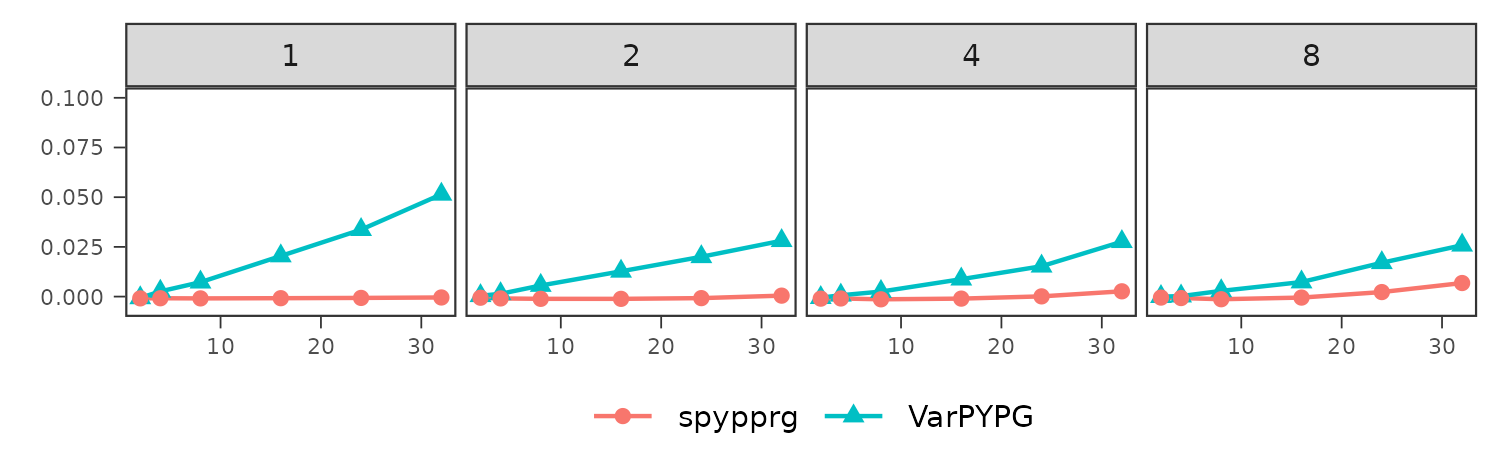
\includegraphics{./plots/energy_score}
\end{figure}

\makenote{need to put in a comparative model to make the variational model not
    look as bad by comparison.}
We see the MCMC model nearly perfectly captures the original distribution as
    measured by energy score.  The variational model is not far behind, however.

% EOF